\documentclass[letterpaper,12pt,oneside]{book}
\usepackage[top=1in, left=1.25in, right=1.25in, bottom=1in]{geometry}
\usepackage{bachelorstitlepageUNAM}

%%%%%%%%%%%%%%%%%%%%%%%%%%%%%
% Comparto una plantilla para la PORTADA que us\'e en mi t\'esis
% basada en el dise\~no gen\'erico que se usa en la Facultad de Ciencias
% Para usarlo \'unicamente aseg\'urate de tener la l\'inea
% \usepackage{bachelorstitlepageUNAM} y el archivo bachelorstitlepageUNAM.sty en el mismo directorio de trabajo.
% y los campos (sin signo %) :
%\author{Nombre del Alumno}
%\title{T\'itulo de la tesis}
%\faculty{Facultad}
%\degree{Grado que obtienes}
%\supervisor{ Tutor}
%\cityandyear{Ciudad y anio}
%\logouni{nombredelescudodelaunamsinespacios}
%\logofac{NombreDeLaImagenDelEscudodeTuFacultadSinEspacios}
% Para sugerencias y comentarios: DM en twitter.com/sglvgdor
% Subir\'e mas adelante la plantilla para maestr\'ia
%%%%%%%%%%%%%%%%%%%%%%%%%%%%%

\author{Pérez Romero Natalia Abigail}
\title{ ...}
\faculty{Facultad de Ciencias}
\degree{Licenciatura en Ciencias de la Computación}
\supervisor{Dr. José David Flores Peñaloza}
\cityandyear{Ciudad Universitaria, Cd. Mx., 2023}
\logouni{Escudo-UNAM}
\logofac{Escudo-FCIENCIAS}

\usepackage[T1]{fontenc}
\usepackage[utf8]{inputenc}
\usepackage[spanish,es-nodecimaldot,es-tabla]{babel}
\usepackage{graphicx}
\usepackage{tikz}
% use hyperref to make the table of contents clickable
\usepackage{hyperref}

\graphicspath{{"imagenes/"}}
\usepackage{setspace}
%\usepackage[round]{natbib}

\usepackage{lipsum}

\begin{document}
\frontmatter
\maketitle

\chapter*{}
\begin{flushright}%
  \emph{Dedicatoria ...}
  \thispagestyle{empty}
\end{flushright}

\chapter{Agradecimientos}
\spacing{1.5}%\doublespacing
%\chapter{Resumen}
%\chapter{Abstract}

\tableofcontents
%\listoffigures

\chapter{Prefacio}

\section*{Contenido de la tesis}
\section*{Panorama general}
\section*{Objetivo}
    
\mainmatter

\chapter{Introducción} %

\section{Protocolo IP} %

El protocolo IP (Internet Protocol) Junto con el protocolo TCP (Transmission Control Protocol) son los dos protocolos más importantes en el Internet.

IP determinará el formato de los paquetes de datos que se envían y reciben a través de la red. TCP se encargará de la transmisión de los datos.

Existen dos versiones de IP, la versión 4 (IPv4) y la versión 6 (IPv6). La versión 4 es la más utilizada en la actualidad, pero se está migrando a la versión 6 debido a la falta de direcciones IP disponibles en la versión 4.

\section{Protocolo TCP} %
El protocolo TCP (Transmission Control Protocol) es un protocolo de transporte orientado a conexión. TCP se encarga de la transmisión de los datos de manera fiable, es decir, garantiza que los datos lleguen a su destino en el orden correcto y sin errores. TCP también se encarga de controlar el flujo de datos, es decir, de evitar que el emisor sature al receptor con datos.

\section{Protocolo UDP} %

El protocolo UDP provee un servicio de transporte no orientado a conexión. UDP es más simple que TCP, ya que no tiene control de flujo, control de errores, ni retransmisión de paquetes.

\section{VPN} %
Las VPN (Virtual Private Network) son redes privadas virtuales que permiten a los usuarios conectarse a una red privada a través de una red pública, como Internet. Las VPN se utilizan para proteger la privacidad y la seguridad de la información transmitida a través de la red.

\section{Wireguard} %
Wireguard es un protocolo de VPN de código abierto y de alto rendimiento. Wireguard es más simple y más rápido que otros protocolos de VPN, como OpenVPN y IPsec.


\section{NAT} %
\section{IP Masquerade} %

\section{Tablas de routeo}  


\section{IPTables} %https://docs.aws.amazon.com/vpc/latest/userguide/VPC_Route_Tables.html
IPTables es una herramienta de configuración de firewall en sistemas operativos basados en Linux. Entre sus funciones se encuentran el filtrado de paquetes, redireccionamiento de paquetes, traducción de direcciones de red, etc.


%\section{Firewall} %

\section{Relay network}%


\chapter{Desarrollo}

\section{Casos de uso}
\subsection{Identificación del usuario}

En esta primera version no nos preocuparemos de que la información del usuario se transmita de forma segura, por lo que el usuario deberá ingresar su nombre y contraseña en texto plano. Y se enviará al servidor para su verificación.

\begin{figure}
    \centering
    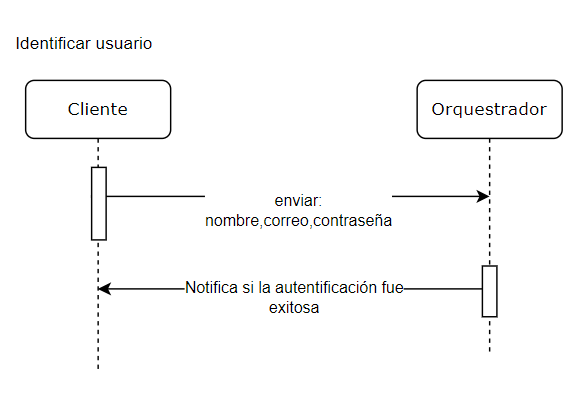
\includegraphics[width=\textwidth]{login-user.png}
    \caption{Pantalla de inicio de sesión}
\end{figure}

\subsubsection{Registro de usuario}

De igual forma el registro de usuario se hará en texto plano, y se enviará al servidor para su verificación.

\begin{figure}
    \centering
    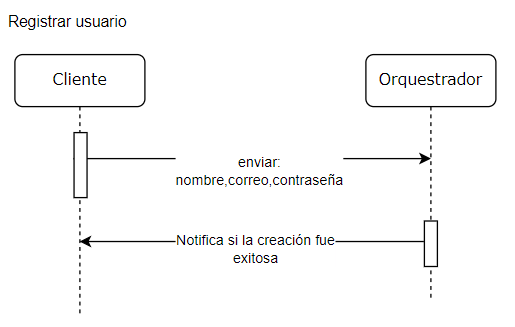
\includegraphics[width=\textwidth]{register-user.png}
    \caption{Pantalla de registro de usuario}
\end{figure}

\subsection{Registro de usuario}

\lipsum[1-2]


\section{Sección}
\lipsum[1-2]

\chapter{Resultados}  %

\chapter{Conclusiones}  %

\bibliographystyle{humannat}
%\bibliography{references}

\backmatter@sglvgdor

% Referencias
%https://www.overleaf.com/learn/latex/Bibliography_management_with_bibtex

\begin{thebibliography}{9}
\bibitem{computerNetworking}
  Kurose, J. F., \& Ross, K. W. (2017).
  \emph{Computer networking: a top-down approach},
  Pearson,
  7th edition.

\bibitem{wireguard}
    WireGuard,
    \emph{WireGuard: fast, modern, secure VPN tunnel},
    \url{https://www.wireguard.com/},
    2021.

\bibitem{linuxNetworkingGuide}
    Linux Documentation Project,
    \emph{Linux Advanced Routing \& Traffic Control HOWTO},
    \url{https://tldp.org/HOWTO/Adv-Routing-HOWTO/index.html},
    2021.

\bibitem{networkAdministartionGuide}
    Bautts, M., \& Dawson, M. (2000).
    \emph{Linux Network Administrator's Guide},
    O'Reilly Media,
    3rd edition.

% https://tldp.org/HOWTO/IP-Masquerade-HOWTO/kernel-2.4.x-requirements.html

\bibitem{ipMasquerade}
    Bautts, M., \& Dawson, M. (2000).
    \emph{Linux IP Masquerade HOWTO},
    \url{https://tldp.org/HOWTO/IP-Masquerade-HOWTO/index.html},
    2021.

\end{thebibliography}

\end{document}